\documentclass[12pt,letter]{article}

%% \usepackage[fleqn]{amsmath}
\usepackage[margin=1in]{geometry}
\usepackage{amsmath,amsfonts,amsthm,bm}
\usepackage{breqn}
\usepackage{amsmath}
\usepackage{amssymb}
\usepackage{tikz}
\usepackage{algorithm2e}
\usepackage{siunitx}
\usepackage{graphicx}
\usepackage{subcaption}
%% \usepackage{datetime}
\usepackage{multirow}
\usepackage{multicol}
\usepackage{mathrsfs}
\usepackage{fancyhdr}
\usepackage{fancyvrb}
\usepackage{parskip} %turns off paragraph indent
\usepackage{float}
\usepackage{empheq}

\pagestyle{fancy}

\usetikzlibrary{arrows}

\DeclareMathOperator*{\argmin}{argmin}
\newcommand*{\argminl}{\argmin\limits}

\newcommand{\mathleft}{\@fleqntrue\@mathmargin0pt}
\newcommand{\R}{\mathbb{R}}
\newcommand{\Z}{\mathbb{Z}}
\newcommand{\N}{\mathbb{N}}
\newcommand{\ppartial}[2]{\frac{\partial #1}{\partial #2}}
\newcommand{\norm}[1]{\|#1\|}
\newcommand{\set}[1]{\{#1\}}
\newcommand{\notimplies}{\;\not\!\!\!\implies}

\setcounter{MaxMatrixCols}{20}

\begin {document}

  % \begin{cases}
  %     0, & \text{if}\ a=1 \\
  %     1, & \text{otherwise}
  %   \end{cases}

\lhead{Convex Optimization - HW3}
\rhead{(Bill) Yuan Liu, 996954078, 2020/03/16}

\begin{enumerate}
\item Q 5.12 textbook\\
  Derive dual problem for: $min_x - \sum_i log(b_i-a_i^Tx), x: a_i^Tx < b_i, \forall i \in \{1,..,m\}$
  \begin{align*}
    &let\ y_i = b_i-a_i^Tx > 0\\
    &a_i^Tx < b_i\ relax\ to\ a_i^Tx \leq b_i\\
    &L(x,y,\lambda,v)=-\sum_i log y_i + \sum_i \lambda_i(a_i^Tx-b_i) + \sum_i v_i(y_i+a_i^Tx-b_i)\\
    &g(\lambda,v)=\inf_{x,y} L(x,y,\lambda,v)\\
    &g(\lambda,v)=\inf_{x,y}-\sum_i log y_i + \sum_i \lambda_i(a_i^Tx-b_i) + \sum_i v_i(y_i+a_i^Tx-b_i)\\
    &(\exists i)\lambda_i > 0 \wedge a_i^Tx - b_i < 0 \implies \lambda_i(a_i^Tx-b_i)\ unbounded,\ so\ \lambda \leq 0\\
    &\lambda \geq 0 \wedge \lambda \leq 0 \implies \lambda = 0\\
    &g(\lambda,v)=\inf_{x,y}-\sum_i log y_i + \sum_i v_i(y_i+a_i^Tx-b_i)\\
    &g(\lambda,v)=\inf_{x,y}-\sum_i log y_i + v^Ty + v^TAx - v^Tb\\
    &y_i > 0 \implies -log y_i\ decreasing\\
    &y_i > 0 \wedge (\exists v_i < 0) \implies \inf_{y_i} -log y_i + v_i y_i\ \to -\infty,\ so\ v \succeq 0\\
    &\frac{\partial}{\partial y_i}(-\sum_i log y_i + v^Ty + v^TAx - v^Tb)=-\frac{1}{y_i} + v_i=0\\
    &(\forall i) \frac{\partial}{\partial y_i}(-\frac{1}{y_i} + v_i)>0 \implies convexity\\
    &y_i = \frac{1}{v_i}, v_i \neq 0\\
    &(\forall i) v_i \neq 0 \wedge v_i \geq 0 \implies v \succ 0\\
    &\frac{\partial}{\partial x}(-\sum_i log y_i + v^Ty + v^TAx - v^Tb)=A^Tv=0\\
    &g(\lambda,v)=
      \begin{cases}
        -\sum_i log \frac{1}{v_i} + \sum_i \frac{v_i}{v_i} - v^Tb, & \text{if } A^Tv=0 \wedge v \succ 0\\
        -\infty, & \text{otherwise}
      \end{cases}
  \end{align*}
  Dual problem:
  \begin{align*}
    \max_{\lambda,v} &\sum_i log v_i + m - v^Tb = -(\min_{\lambda,v}-\sum_i log v_i - m + v^Tb)\\
    s.t.\ &A^Tv = 0\\
    &-v_i \leq 0, \forall i\\
  \end{align*}
  \pagebreak
\item Q 5.27 Equality constrained least squares\\
  Give KKT conditions, derive expressions for primal and dual solutions.
  \begin{align*}
    \min_x & \norm{Ax-b}_2^2\\
    s.t.\ & Gx=h            
  \end{align*}
  \begin{align*}
    &affine\ equality\ constraints\ only \implies Slater's\ condition\ satisfied\\
    &f_0 = x^TA^TAx + 2b^TAx + b^Tb\\
    &h_0 = Gx-h\\
    &L(x,\lambda,v) = f_0 + v^Th_0\\
    &L(x,\lambda,v) = x^TA^TAx - 2b^TAx + b^Tb + v^T(Gx-h)\\
    &\frac{\partial L}{\partial x^*} = 0 = 2A^TAx^* - 2A^Tb + G^Tv\\
    \\
    &KKT\ conditions:\\
    &x^* = \frac{1}{2}(A^TA)^{-1}(2A^Tb - G^Tv)\\
    &Gx^*-h = 0\\
    \\
    &g(\lambda,v)= \inf_x L(x,\lambda,v) = \frac{1}{4}(2A^Tb-G^Tv)^T(A^TA)^{-1}(2A^Tb-G^Tv)\\
    &-2b^TA(\frac{1}{2}(A^TA)^{-1}(2A^Tb-G^Tv)) + b^Tb + v^T(G\frac{1}{2}(A^TA)^{-1}(2A^Tb-G^Tv)-h)\\
    &g(\lambda,v)= \inf_x L(x,\lambda,v) = \frac{1}{4}(2A^Tb)^T(A^TA)^{-1}(2A^Tb)-(A^Tb)^T(A^TA)^{-1}(G^Tv)\\
    &+\frac{1}{4}(G^Tv)^T(A^TA)^{-1}(G^Tv) +b^TA((A^TA)^{-1}G^Tv)) -h^Tv + v^TG\frac{1}{2}(A^TA)^{-1}(2A^Tb-G^Tv) \\
    &- b^TA(A^TA)^{-1}2A^Tb) + b^Tb\\
    &\text{rid of constants and simplify}:\\
    &g(\lambda,v)= \inf_x L(x,\lambda,v) = -\frac{1}{4}(G^Tv-2A^Tb)^T(A^TA)^{-1}(G^Tv-2A^Tb) \\
    &-\frac{1}{2}(Gv^T)^T(A^TA)^{-1}(G^Tv) -h^Tv\\
  \end{align*}
  Dual problem:
  \begin{align*}
    \max_{\lambda,v} & g(\lambda,v) = \max_v -\frac{1}{4}(G^Tv-2A^Tb)^T(A^TA)^{-1}(G^Tv-2A^Tb) \\
    &-\frac{1}{2}(Gv^T)^T(A^TA)^{-1}(G^Tv) -h^Tv\\
    s,t.\ & Gx^*-h=0
  \end{align*}
  Solve for $v^*$:\\
  \begin{align*}
    &Gx^*-h=0\\
    &x^* = \frac{1}{2}(A^TA)^{-1}(2A^Tb - G^Tv^*)\\
    &G\frac{1}{2}(A^TA)^{-1}(2A^Tb - G^Tv^*)-h=0\\
    &v^*=2G^{-T}(A^Tb-A^TAG^{-1}h)\\
  \end{align*}
  \pagebreak
\item Q 5.35 Sensitivity analysis of GP\\
  After log tranformation:
  \begin{align*}
    &\min_y log f_0(y)\\
    s.t.\ & log f_i(y) \leq 0\\
    & log h_i(y) = 0
  \end{align*}
  Perturbed problem:
  \begin{align*}
    &\min_y log f_0(y)\\
    s.t.\ & log f_i(y) \leq u_i\\
    & log h_i(y) = v_i
  \end{align*}
  where $y_i = log(x_i), x_i > 0$\\
  
  Let $L$:=Lagrangian of original problem after log transform\\
  Let $L'$:=Lagrangian of perturbed problem after log transform\\
  \begin{align*}
    L'(y,\lambda,w) &= log\ f_0(y) + \sum_i \lambda_i(log\ f_i(y)-u_i) + \sum_i w_i(log\ h_i(y) -v_i)\\
    L'(y,\lambda,w) &= L(y,\lambda,w) -\sum_i \lambda_i u_i + -\sum_i w_i v_i\\
    p(u,v) &= \inf_y L'(y,\lambda,w) = \inf_y L(y,\lambda,w) - \lambda^Tu- w^Tv
  \end{align*}
  Dual:
  \begin{align*}
  \max_{\lambda,w} p(u,v) &= p^*(u,v) = \max_{\lambda,w} \inf_y L(y,\lambda,w) - \lambda^Tu- w^Tv\\
    let\ p(0,0) &= \max_{\lambda,w} \inf_y L(y,\lambda,w)\\
    p^*(u,v) &= p(0,0) + (\max_{\lambda,w} -\lambda^Tu- w^Tv)\\
    \lambda & \succeq 0
  \end{align*}
  
  let\ $\lambda^*, w^*$ be parameters for optimal $p(u,v)$
  \begin{align*}
    p^*(u,v) &= p(0,0) -{\lambda^*}^Tu- {w^*}^Tv\\
             u\ not\ present\ &in\ original\ problem \implies \frac{\partial}{\partial u_i}p(0,0) = 0, \forall i\\
             v\ not\ present\ &in\ original\ problem \implies \frac{\partial}{\partial v_i}p(0,0) = 0, \forall i\\
    \frac{\partial}{\partial u_i} p^*(u,v) &= -\lambda_i^*, \forall i\\
    \frac{\partial}{\partial v_i} p^*(u,v) &= -w_i^*, \forall i
  \end{align*}
  Inverse log transform $x \to e^x$ into original form of objective:
  \begin{align*}
    e^{\frac{\partial}{\partial u_i} p^*(u,v)} &= e^{-\lambda_i^*}, \forall i\\
    e^{\frac{\partial}{\partial v_i} p^*(u,v)} &= e^{-w_i^*}, \forall i\\
  \end{align*}
  
  Relaxation of ith constraint by $\alpha$ percent:\\
  $\partial p^*(u_i,0) &= -\lambda_i^*\partial u_i$\\
  $\partial u_i = \alpha \implies$ objective function of log transformed problem experiences a decrease in value by $\lambda_i \alpha$\\
  Converting objective back via inverse of log: $x \to e^{y}$\\
  $z$ small $\implies e^{z} \approx 1+ z$ via Taylor expansion\\
  $e^{-\lambda_i^* \alpha} \approx 1 - \lambda_i^* \alpha, \lambda_i^* \geq 0 \implies$ objective function experiences an improvement of $\lambda_i^* \alpha$ percent since it is a minimization problem.\\
  \pagebreak
\item Q 5.42. Find Lagrange dual problem in inequality form.
  \begin{align*}
    \min_x\ & c^Tx\\
    s.t.\ & Ax \preceq_K b\\
  \end{align*}
  \begin{align*}
    L(x,\lambda,v) & = c^Tx + \lambda^T(Ax-b)\\
    \lambda & \succeq_{K^*} 0\\
    g (\lambda,v) &= \inf_x L(x,\lambda,v)\\
    g (\lambda,v) &=
                    \begin{cases}
                      -\lambda^Tb, & c + A^T\lambda = 0\\
                      -\infty, & o/w
                    \end{cases}
  \end{align*}
  Dual:
  \begin{align*}
    \max_{\lambda,v}\ & g(\lambda,v) = \max_{\lambda}\ -b^T\lambda\\
    s.t.\ & c+A^T\lambda = 0\\
    \lambda & \succeq_{K^*} 0\\
    \\
    let\ y & = -\lambda\\
    \\
    \max_{y}&\ b^Ty\\
    s.t.\ & A^Ty = c\\
    y & \preceq_{K^*} 0\\
  \end{align*}
  \pagebreak
\item Strong Duality for LP:\\
  Primal:
  \begin{align*}
    \min_x\ & c^Tx\\
    s.t.\ & Ax \geq b\\
           & x \geq 0
  \end{align*}
  Find the dual of the primal and argue that
  \begin{itemize}
  \item a) if the primal is unbounded then the dual is infeasible
    \begin{align*}
      L(x,\lambda,v) &= c^Tx + \lambda_1^T(b-Ax) + \lambda_2^T(-x)\\
      L(x,\lambda,v) &= (c^T-\lambda_1^TA -\lambda_2^T)x + \lambda_1^Tb\\
      g(\lambda,v) &= \inf_x L(x,\lambda,v) =
      \begin{cases}
        b^T\lambda_1, & c -A^T\lambda_1-\lambda_2 = 0\\
        -\infty, & o/w
      \end{cases}\\
      Dual:\\
      \max_{\lambda_1,\lambda_2}\ & b^T\lambda_1\\
      s.t.\ & c - A^T\lambda_1 - \lambda_2 = 0\\
      \lambda_1 & \geq 0\\
      \lambda_2 & \geq 0
    \end{align*}
  \begin{align*}
    &g(\lambda,v) \leq c^Tx^*\\
    &primal\ unbounded:\ c^Tx^*= -\infty \implies g(\lambda,v) = -\infty \implies\\
    &c -A^T\lambda_1-\lambda_2 \neq 0 \implies infeasible\ case\ of\ dual
  \end{align*}
  \pagebreak
\item b) if the primal is infeasible then the dual is either infeasible or unbounded\\
  
  primal infeasible:
    \begin{align*}
      &(\exists i) (b-Ax)_i > 0 \vee (\exists i) (-x)_i > 0\\
      \\
      &g(\lambda_1,\lambda_2) = \inf_x c^Tx +\lambda_1^T(b-Ax) + \lambda_2^T(-x) \leq c^Tx\\
      &\lambda_1 \succeq 0\\
      &\lambda_2 \succeq 0\\
      % &g(\lambda_1,\lambda_2) = c^Tx^* +\lambda_1^T(b-Ax^*) + \lambda_2^T(-x^*) \leq c^Tx^*\\
      &g(\lambda_1,\lambda_2) = \inf_x c^Tx +\lambda_1^T(b-Ax) + \lambda_2^T(-x)\\
      &dual: \max_{\lambda_1,\lambda_2} g(\lambda_1,\lambda_2)\\
      % &let\ x^*\ be\ optimal,\ disregarding\ infeasibility\ of\ the\ primal\\
      &let\ x^*\ be\ optimal\ for\ g(\lambda_1,\lambda_2) = c^Tx^* +\lambda_1^T(b-Ax^*) + \lambda_2^T(-x^*)\\
      &if\ x^*\ is\ primal\ infeasible:\\
      &\lambda_1 \succeq 0, \lambda_2 \succeq 0 \wedge (\exists i) (b-Ax^*)_i > 0 \wedge \lambda_{1_i} \to +\infty \implies \max_{\lambda_1, \lambda_2} g(\lambda_1,\lambda_2) \to +\infty\\
      &\lambda_1 \succeq 0, \lambda_2 \succeq 0 \wedge (\exists i) (-x^*)_i > 0 \wedge \lambda_{2_i} \to +\infty \implies \max_{\lambda_1, \lambda_2} g(\lambda_1,\lambda_2) \to +\infty\\
      &dual\ is\ unbounded\ in\ this\ case\\
      \\
      &suppose\ optimal\ value\ of\ dual\ exists\ with:\\
      &\max_{\lambda_1,\lambda_2} c^Tx^* +\lambda_1^T(b-Ax^*) + \lambda_2^T(-x^*) = c^Tx^*\\
      &c^Tx^* +\lambda_1^*^T(b-Ax^*) + \lambda_2^*^T(-x^*) = c^Tx^*\\
      &\lambda_1^*^T(b-Ax^*) + \lambda_2^*^T(-x^*) = 0\\
      &primal\ infeasibility\ enforces:\\
      &(\exists i)(b-Ax)_i > 0 \vee (\exists i)(-x)_i > 0\\
      &suppose:\\
      &(\exists i)(b-Ax)_i > 0 \wedge (-x)_i < 0 \implies\\
      &\lambda_1^*^T(b-Ax^*)_i + \lambda_2^*^T(-x^*)_i = 0,\ where\ \lambda_{1_i}^* = -\alpha \lambda_{2_i}^*, \alpha > 0\\
      % &\lambda_1, \lambda_2\ can\ be\ unbounded\ below,\ not\ satisfying\ dual\ feasibility:\ \lambda_1 \not\succeq 0 \vee \lambda_2 \not\succeq 0\\
      &suppose:\\
      &(\exists i,j,i\not=j)(b-Ax)_i > 0 \wedge (b-Ax)_j > 0 \wedge (b-Ax)_i = 0, (b-Ax)_j = 0\implies\\
      &\lambda_1^*^T(b-Ax^*)_i + \lambda_1^*^T(b-Ax^*)_j = 0,\ where\ \lambda_{1_i}^* = -\alpha \lambda_{1_j}^*, \alpha > 0\\
      &similiarily\ for:\ (\exists i,j)(b-Ax)_i > 0 \wedge (-x)_j > 0\ and\ (\exists i,j,i\not=j)(-x)_i > 0 \wedge (-x)_j > 0\\
      \\
      &\lambda_1,\lambda_2\ can\ be\ chosen\ such\ that\ \lambda_1 \not\succeq 0 \vee \lambda_2 \not\succeq 0,\ thus\ not\ satisfying\ dual\ feasibility.\\
    \end{align*}
  \end{itemize}
  \pagebreak
\item Game Theory
  \begin{align*}
    &\min_x \max_y x^TPy\\
    s.t.\ &Ax \leq b\\
    &Cy \leq d
  \end{align*}
  \begin{align*}
      &\max_y \min_x x^TPy\\
      s.t.\ &Ax \leq b\\
      &Cy \leq d
    \end{align*}
  \begin{enumerate}
  \item show that min-max problem as the same optimal value as the following minimization problem:
    \begin{align*}
      &\min_{\lambda,x} d^T \lambda\\
      s.t.\ & C^T \lambda = P^Tx\\
      &Ax \leq b\\
      &\lambda \geq 0
    \end{align*}
    Inner optimization problem:
    \begin{align*}
      \max_y & (P^Tx)^T y = -(\min_y -(P^Tx)^T y)\\
      s.t.\ &Ax \leq b\\
             &Cy \leq d\\
      g(\lambda_1,\lambda_2) & = \inf_y -(P^Tx)^T y =
                           \begin{cases}
                             \lambda_1^T(Ax-b)-\lambda_2^Td, & -P^Tx+C^T\lambda_2 = 0\\
                             -\infty, & o/w
                           \end{cases}\\
      \max_{\lambda_1,\lambda_2}\ & g(\lambda_1,\lambda_2) = \max_{\lambda_1,\lambda_2} -\lambda_2^Td + \lambda_1^T(Ax-b)\\
      s.t.\ & -P^Tx+C^T\lambda_2 = 0\\
             &\lambda_1, \lambda_2 \geq 0\\
             & \lambda_1^T(Ax-b) \leq 0 \implies\\
      \max_{\lambda_1,\lambda_2}\ & g(\lambda_1,\lambda_2) = \max_{\lambda_2} -\lambda_2^Td\\
      -(\min_y & -(P^Tx)^T y) = - \max_{\lambda_1,\lambda_2} g(\lambda_1,\lambda_2) = -(-\min_{\lambda_2} \lambda_2^Td) = \min_{\lambda_2} \lambda_2^Td\\
             rename\ &\lambda_2\ to\ \lambda\ and\ enclose\ with\ outer\ minimization\ over\ x:\\
      \min_{x,\lambda}&\ \lambda^Td\\
      s.t.\ &P^Tx = C^T\lambda\\
             &Ax \leq b\\
             &\lambda \geq 0
    \end{align*}
    \pagebreak
  \item show that max-min problem as the same optimal value as the following maximization problem:
    \begin{align*}
      &\max_{y,v} -b^T v\\
      s.t.\ & A^Tv + Py = 0\\
      &Cy \leq d\\
      &v \geq 0
    \end{align*}
    Inner optimization problem:
    \begin{align*}
      \min_x &\ x^TPy\\
      s.t.\ &Ax \leq b\\
             &Cy \leq d
      \\
      g(\lambda_1,\lambda_2) & = \inf_x x^TPy + \lambda_1^T(Ax-b) + \lambda_2^T(Cy-d)\\
      & =
        \begin{cases}
          -\lambda_1^Tb + \lambda_2^T(Cy-d), & Py + A^T\lambda_1 = 0\\
          - \infty, & o/w
        \end{cases}\\
      max_{\lambda_1,\lambda_2} g(\lambda_1,\lambda_2) & = \max_{\lambda_1,\lambda_2} -\lambda_1^Tb + \lambda_2^T(Cy-d)\\
      s.t.\ & P^Ty + A^T\lambda_1 = 0\\
      &\lambda_1 \geq 0\\
      &\lambda_2 \geq 0\\
      % &Ax-b \leq 0\\
      &Cy-d \leq 0 \implies \lambda_2^T(Cy-d)  \leq 0 \implies\\
      \max_{\lambda_1,\lambda_2} & \ g(\lambda_1,\lambda_2) = \max_{\lambda_1,\lambda_2} -\lambda_1^Tb\\
      s.t.\ & P^Ty + A^T\lambda_1 = 0\\
      &\lambda_1 \geq 0\\
             &Cy-d \leq 0\\
             &rename\ variables\ and\ enclose\ with\ outer\ optimization:\\
      \max_{y,v} &-b^Tv\\
      s.t.\ &P^T y + A^Tv = 0\\
      Cy &\leq d\\
      v &\geq 0
    \end{align*}
  \item show the above problems have the same optimal value (min-max equals max-min)
    \begin{align*}
      \min_{x,\lambda}&\ d^T \lambda\\
      s.t.\ & C^T\lambda = P^T x\\
                       &Ax \leq b\\
                       &\lambda \geq 0\\
      \\
      g(a_1,a_2,w) &= \inf_{x,\lambda} d^T\lambda + a_1^T(Ax-b)+a_2^T(-\lambda) + w^T(C^T\lambda-P^Tx)\\
      s.t.\ &a_1 \geq 0\\
                       &a_2 \geq 0\\
      % &Ax-b \leq 0\\
                       % &-\lambda \leq 0\\
                       % &C^T\lambda - P^Tx = 0\\
      g(a_1,a_2,w) &=
                     \begin{cases}
                       -a_1^Tb , & d-a_2+Cw=0 \wedge A^Ta_1-Pw=0\\
                       -\infty, & o/w
                     \end{cases}\\
      Dual:&\\
      \max_{a_1,a_2,w}\ & g(a_1,a_2,w) = -b^Ta_1\\
      s.t.\ & d-a_2+Cw=0\\
                      &A^Ta_1-Pw=0\\
                      &a_2 \geq 0 \implies d+Cw \geq 0\\
                      &a_1 \geq 0\\
      \\
      let\ &v = a_1, y = -w\\
      \max_{v,y}&\ g(v,y) = -b^Tv\\
      s.t.\ &A^Tv+Py=0\\
                      &Cy \leq d\\
                      &v \geq 0\\
    \end{align*}
    We start with equivalent formulation of min-max and arrive at a equivalent formulation of max-min problem thus they obtain the same optimal value.
  \end{enumerate}
  \pagebreak
  
\item Optimal control of a unit mass revisited\\
  \begin{align*}
    \norm{p}_1 = \sum_{i=1}^{10} |p_i|\\
    \norm{p}_{\infty} = \max_{i=1,..,10} |p_i|
  \end{align*}
  \begin{enumerate}
  \item Consider $\norm{p}_1$ problem with same setup in Q9(1) of last assignment. Find optimal solution. Plot optimal force, position, and velocity. Write down the primal and dual solutions.
    \begin{align*}
      \min_p \sum_{i=1}^{10} |p_i|
    \end{align*}
    Constraints: $x(0)=0,x(10)=1,\dot{x}(0)=0,v(0)=0,v(10)=0$\\
    let $v=\dot{x}$
    \begin{align*}
      v(i) &= v(0) + \sum_{j=1}^i p_j/m,m=1\\
      v(10) &= \sum_{j=1}^i p_j = 0\\
      x(i) &= x(0) + \sum_{j=0}^i v(j)\\
      x(i) &= \sum_{j=1}^i \sum_{k=1}^j p_k = \sum_{j=1}^i (i-j+1)p_j\\
      x(10) &= [10,9,..,1]p=1
    \end{align*}
    Primal:
    \begin{align*}
      let\ t_i &= |p_i|\\
      let\ X &= [p_1,..,p_{10}, t_1,..,t_{10}]^T\\
      \min_X &
      \begin{bmatrix}
        1_{1:10}^T & 0_{1:10}^T
      \end{bmatrix} X\\
      s.t.\ 
        &\begin{bmatrix}
          1^T & 0^T\\
          10,9,..1 & 0^T
        \end{bmatrix} X
                     =
                     \begin{bmatrix}
                       0 \\ 1
                     \end{bmatrix}\\
      &\begin{bmatrix}
        I_{10\times 10} & -I_{10\times 10}\\
        -I_{10\times 10} & -I_{10\times 10}
      \end{bmatrix}X \leq
                           \begin{bmatrix}
                             0_{20 \times 1}
                           \end{bmatrix}
    \end{align*}
    \pagebreak
    \begin{align*}
      L(p,t,\lambda,v) &= 1^T t + \lambda_1^T(p-t)+\lambda_2^T(-p-t)+v_1^T(1^Tp) + v_2^T([10..1]p-1)\\
                       &= (1^T-\lambda_1^T-\lambda_2^T)t+(\lambda_1^T-\lambda_2^T+v_2^T[10..1] + v_1^T1^T)p -v_2^T1\\
      g(\lambda,v) &= \inf_{p,t} L(p,t,\lambda,v)\\
                       &=
                         \begin{cases}
                           -v_2, & 1-\lambda_1-\lambda_2=0, \lambda_1-\lambda_2+[10..1]^T v_2 + 1v_1 =0\\
                           -\infty, & o/w
                         \end{cases}
    \end{align*}
    \begin{align*}
      \max_{\lambda,v}&\ -v_2\\
      s.t.\ &1-\lambda_1-\lambda_2 = 0\\
                      &\lambda_1-\lambda_2 +
                        \begin{bmatrix}
                          10 \\ ..\\ 1
                        \end{bmatrix}v_2 + 1_{10\times 1}v_1 = 0\\
      \lambda_1 &\geq 0\\
      \lambda_2 &\geq 0
    \end{align*}
    Dual:
    \begin{align*}
      &let\ X=[\lambda_1, \lambda_2, v_1, v_2]^T\\
      &\lambda_1, \lambda_2 \in \R^{10}\\
      &v_1,v_2 \in R\\
      \max_{X}&\
                \begin{bmatrix}
                  0^T & 0^T & 0 & -1
                \end{bmatrix}X\\
      s.t.\ &
              \begin{bmatrix}
                I_{10\times 10} & -I_{10\times 10} & 1_{10\times 1} & [10..1]^T& \\
                I_{10\times 10} & I_{10\times 10} & 0 & 0
              \end{bmatrix}X =
                                                          \begin{bmatrix}
                                                            0_{10\times 1}\\
                                                            1_{10\times 1}
                                                          \end{bmatrix}\\
      &\begin{bmatrix}
        -I & -I & 0 & 0
      \end{bmatrix} X \leq 0
    \end{align*}
    Solve using Matlab:\\
    $cost_{optimal}=0.2222$\\
    Primal solution:\\
    $p(1)=0.1111, p(10)=-0.1111, (\forall i \not\in \{1,10\})\ p(i)=0$\\
    $t(1)=t(10)=0.1111, (\forall i \not\in \{1,10\})\ t(i)=0$\\
    
    Dual solution:\\
    $\lambda_1 = [1,0.8889,0.7778,0.6667,0.5556,0.4444,0.3333,0.2222,0.1111,0]$\\
    $\lambda_2 = [0, 0.1111, 0.2222, 0.3333, 0.4444, 0.5556, 0.6667, 0.7778, 0.8889, 1]$\\
    $v_1=1.2222, v_2 =-0.2222$\\
    
    \begin{figure}[H]
    \centering
    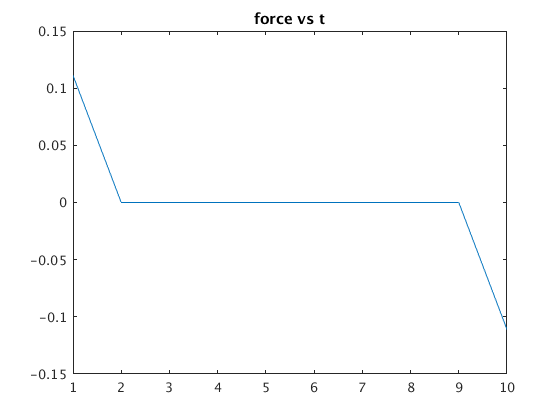
\includegraphics[width=10cm]{q7/q7_a_1.png}
    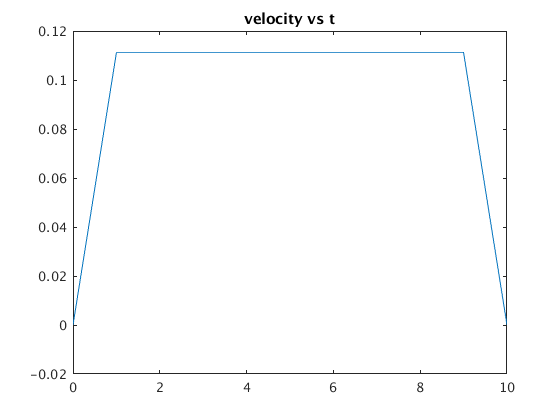
\includegraphics[width=10cm]{q7/q7_a_2.png}
    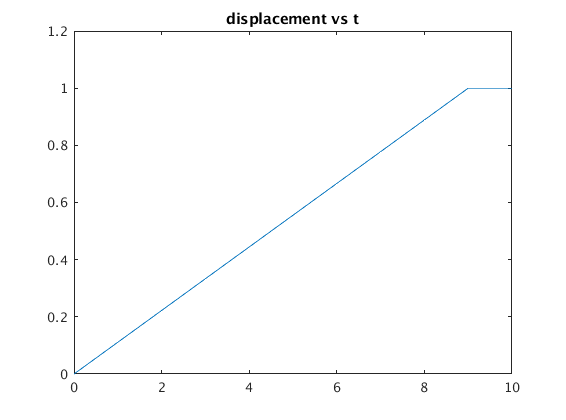
\includegraphics[width=10cm]{q7/q7_a_3.png}
  \end{figure}

\begin{verbatim}
%% part a
f = [zeros(10,1); ones(10,1)]
A = [eye(10) -eye(10); -eye(10) -eye(10)]
b= [zeros(20,1)]

Aeq = [ones(1,10) zeros(1,10); 10:-1:1 zeros(1,10)]
beq = [0;1]
[xs,fval,exitflag,output,lambda] = linprog(f,A,b,Aeq,beq)

force = xs(1:10)
plot(1:10,force)
title('force vs t')

v = zeros(11,1)
for i=2:1:11
    v(i) = v(i-1) + force(i-1)
end

plot(0:1:10,v)
title('velocity vs t')

x = zeros(11,1)
for i=1:1:11
    if i > 1
        x(i) = x(i-1) + v(i)
    else
        x(i) = v(i)
    end
end

plot(0:1:10,x)
title('displacement vs t')
\end{verbatim}
    \pagebreak
  \item
    \begin{enumerate}
    \item Verify that for any vector $v$ and $w$, we always have $|w^Tv| \leq \norm{v}_{\infty} \norm{w}_1$
      \begin{align*}
        |w^Tv| &= |\sum_i w_i v_i| \leq \sum_i |w_i v_i| \leq  \sum_i |w_i|v', v' = \max_i |v_i|\\
        |w^Tv| &\leq v' \sum_i |w_i| = \norm{v}_{\infty} \norm{w}_1
      \end{align*}
    \item Let $z$ be any solution of $Az=y$, explain why for any $\lambda$, we must have
      \begin{align*}
        \norm{z}_1 \geq \frac{|\lambda^Ty|}{\norm{A^T\lambda}_{\infty}}
      \end{align*}
      and thus $z,\lambda$ for which the above inequality is satisfied with equality means $z$ must be optimal.
      \begin{align*}
        \frac{|\lambda^Ty|}{\norm{A^T\lambda}_{\infty}} &= \frac{|\lambda^TAz|}{\norm{A^T\lambda}_{\infty}}=\frac{|z^TA^T\lambda|}{\norm{A^T\lambda}_{\infty}}\\
        |z^TA^T\lambda| &\leq \norm{z}_1 \norm{A^T\lambda}_{\infty}\\
        \frac{|\lambda^Ty|}{\norm{A^T\lambda}_{\infty}} &\leq \frac{\norm{z}_1 \norm{A^T\lambda}_{\infty}}{\norm{A^T\lambda}_{\infty}}\\
        \frac{|\lambda^Ty|}{\norm{A^T\lambda}_{\infty}} &\leq \norm{z}_1\\
      \end{align*}
    \item Set $\lambda$ to be the Lagrange multiplier associated with the equality constraint in part (a). Use the above inequality to directly verify that the bang-bang solution is optimal.
      \begin{align*}
        &AX=y\\
        &\begin{bmatrix}
          1^T & 0^T\\
          10,9,..1 & 0^T
        \end{bmatrix} X
                     =
                     \begin{bmatrix}
                       0 \\ 1
                     \end{bmatrix}\\
        &let\ \lambda = [v_1, v_2]^T=[1.2222,-0.2222]^T\\
        &\norm{X}_1 = \norm{[p_1,...,p_{10},t_1,..,t_{10}]}_1 = 0.1111-0.1111+0.1111+0.1111=0.2222\\
        &|\lambda^T y| = \bigg|\lambda^T
          \begin{bmatrix}
            0\\1
          \end{bmatrix}\bigg| = 0.2222\\
        &\|A^T \lambda\|_{\infty} = \bigg\|\begin{bmatrix}
          1^T & 0^T\\
          10,9,..1 & 0^T
        \end{bmatrix}^T \lambda\bigg\|_{\infty} = 1\\
        &\frac{|\lambda^T y|}{\norm{A^T\lambda}_{\infty}} = 0.2222 = \norm{X}_1\\
        &tight\ inequality \implies X\ is\ optimal
      \end{align*}
      
    \end{enumerate}
    \pagebreak
  \item Repeat part (a) for $\norm{\ast}_{\infty}$ minimization problem.
    \begin{align*}
      \min_{p} \norm{p}_{\infty}
    \end{align*}
    \begin{align*}
      let\ t&=\max_i |p_i|\\
      \min_{p,t}\ & t\\
      s.t.\ & p_i \leq t, \forall i\\
                 & p_i \geq -t, \forall i\\
                 &1^Tp=0\\
                 &[10,..,1]p = 1
    \end{align*}
    Primal:
    \begin{align*}
      &let\ X=[p,t]^T\\
      &p\in\R^{10},t\in\R\\
      \min_{X}\ &
                  \begin{bmatrix}
                    0^T & 1
                  \end{bmatrix} X\\
      s.t.\ &
              \begin{bmatrix}
                1^T & 0\\
                10..1 & 0
              \end{bmatrix} X =
                        \begin{bmatrix}
                          0\\1
                        \end{bmatrix}\\
      &
        \begin{bmatrix}
          I & -1_{10\times 1}\\
          -I & -1_{10\times 1}
        \end{bmatrix} \leq 0_{20\times 1}
    \end{align*}
    \pagebreak
    \begin{align*}
      L(p,t,\lambda,v) &= t + \lambda_1^T(p-t) + \lambda_2^T(-p-t) + v_1^T1^Tp + v_2^T([10,..,1]p-1)\\
      g(\lambda,v) &= \inf_{p,t} L(p,t,\lambda,v)\\
                       &=
                         \begin{cases}
                           -v_2, & \lambda_1 - \lambda_2 + 1v_1 + [10,..,1]^Tv_2 = 0, 1-1^T\lambda_1-1^T\lambda_2 = 0\\
                           -\infty, & o/w
                         \end{cases}
    \end{align*}
    Dual:
    \begin{align*}
      &let\ X = [\lambda_1,\lambda_2,v_1,v_2]^T\\
      \max_{X} &
                 \begin{bmatrix}
                   0^T & 0^T & 0 & -1
                 \end{bmatrix}X\\
      s.t.\ &
              \begin{bmatrix}
                I_{10\times 10} & -I_{10\times 10} & 1_{10\times 1} & [10..1]^T\\
                -1^T & -1^T & 0 & 0
              \end{bmatrix}X =
                                  \begin{bmatrix}
                                    0_{10\times 1}\\
                                    -1
                                  \end{bmatrix}\\
      &\begin{bmatrix}
        -I_{10\times 10} & 0_{10\times 10} & 0_{10\times 2}\\
        0_{10\times 10} & -I_{10\times 10} & 0_{10\times 2}
      \end{bmatrix} X \leq 0_{20\times 1}
    \end{align*}
    Solve using Matlab:\\
    $cost_{optimal}=0.04$\\
    Primal solution:\\
    $(\forall i \in \{1,..,5\})\ p(i)=0.04$\\
    $(\forall i \in \{6,..,10\})\ p(i)=-0.04$\\
    $t=0.04$\\
    
    Dual solution:\\
    $\lambda_1 = [0.2,0.16,0.12,0.08,0.04,0,0,0,0,0]$\\
    $\lambda_2 = [0,0,0,0,0,0,0.04,0.08,0.12,0.16]$\\
    $v_1=0.2, v_2 =-0.04$

    \begin{figure}[H]
    \centering
    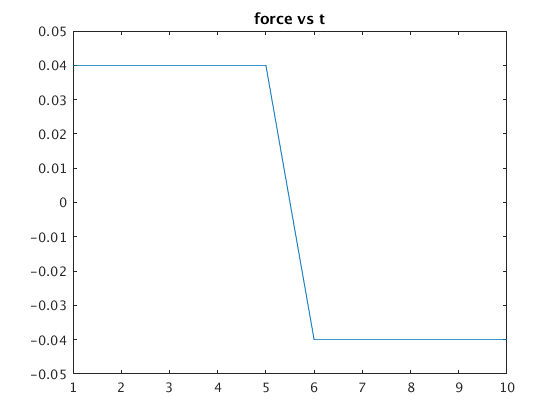
\includegraphics[width=10cm]{q7/q7_c_1.png}
    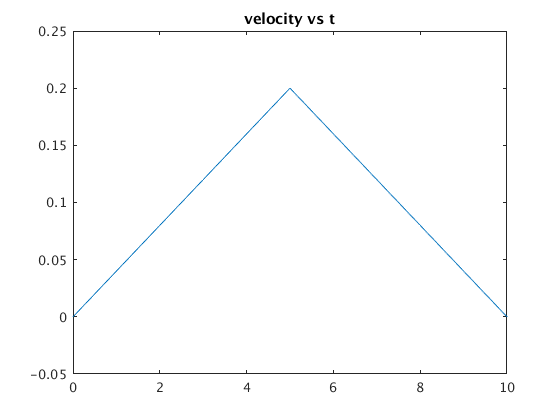
\includegraphics[width=10cm]{q7/q7_c_2.png}
    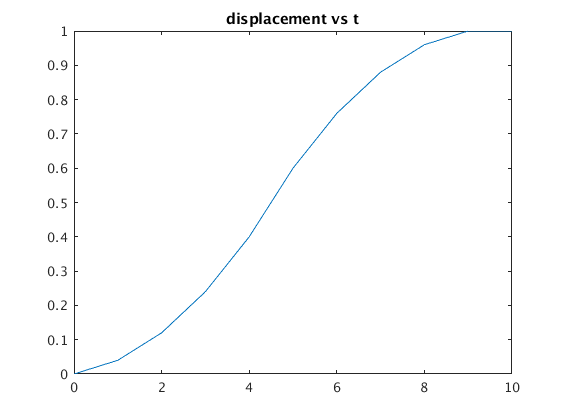
\includegraphics[width=10cm]{q7/q7_c_3.png}
  \end{figure}

\begin{verbatim}
%% part c
f = [zeros(10,1); 1]
A = [eye(10) -ones(10,1); -eye(10) -ones(10,1)]
b= [zeros(20,1)]

Aeq = [ones(1,10) 0; 10:-1:1 0]
beq = [0;1]
[xs,fval,exitflag,output,lambda] = linprog(f,A,b,Aeq,beq)

force = xs(1:10)
plot(1:10,force)
title('force vs t')

v = zeros(11,1)
for i=2:1:11
    v(i) = v(i-1) + force(i-1)
end

plot(0:1:10,v)
title('velocity vs t')

x = zeros(11,1)
for i=1:1:11
    if i > 1
        x(i) = x(i-1) + v(i)
    else
        x(i) = v(i)
    end
end

plot(0:1:10,x)
title('displacement vs t')
\end{verbatim}
  \end{enumerate}
  
\end{enumerate}

\end {document}
